\documentclass[border=3pt]{standalone}
% Preâmbulo compartilhado pelos diagramas TikZ da aula 8 de IHR (Métodos de Pesquisa)
\usepackage[T1]{fontenc}
\usepackage[utf8]{inputenc}
\usepackage{lmodern}
\usepackage{amsmath}
\usepackage{xcolor}
\usepackage{tikz}
\usetikzlibrary{arrows.meta,angles,quotes,decorations.pathmorphing,decorations.pathreplacing,calc,
                positioning,shapes.geometric,shapes.misc,backgrounds,fit,
                math}

% Paleta (mesma dos SVGs originais)
% Paleta da disciplina de IHR: acento azul (#1A6FB5), cor de destaque do tema.
% (o nome "dblue" é mantido para não alterar todos os diagramas)
\definecolor{dblue}{HTML}{1A6FB5}
\definecolor{dorange}{HTML}{B3541E}
\definecolor{dgreen}{HTML}{4A7C59}
\definecolor{dred}{HTML}{9C4B4B}
\definecolor{dcream}{HTML}{F4F1EA}
\definecolor{dshade}{HTML}{DDD7C9}

% Função gaussiana (não normalizada por padrão de escala visual)
\pgfmathdeclarefunction{gauss}{3}{%
  \pgfmathparse{1/(#3*sqrt(2*pi))*exp(-((#1-#2)^2)/(2*#3^2))}%
}

% Estilos comuns (prefixo d... para não colidir com chaves internas do pgf)
\tikzset{
  >={Stealth[length=2mm]},
  dguide/.style={gray!55, dashed, line width=0.4pt},
  daxis/.style={gray!60, line width=0.7pt, ->},
  dbody/.style={fill=black!3, draw=black!80, line width=1pt},
  dacc/.style={draw=dblue, line width=1pt},
  dlbl/.style={black!55, font=\small},
  dsub/.style={black!45, font=\footnotesize},
  dstate/.style={circle, draw=black!80, fill=dcream, line width=1pt,
                 minimum size=17mm, font=\large, inner sep=1pt},
  dobs/.style={circle, draw=black!80, fill=dshade, line width=1pt,
               minimum size=14mm, font=\large, inner sep=1pt},
  dbox/.style={rounded corners=2pt, draw=black!80, fill=dcream, line width=1pt,
               align=center, inner sep=6pt},
  dop/.style={circle, draw=black!80, fill=white, line width=1pt,
              minimum size=6mm, inner sep=0pt, font=\small},
  dtrans/.style={->, dblue, line width=1pt},
  dmeas/.style={->, dorange, line width=1pt},
  dcurve/.style={line width=1pt, dblue},
  dcurveb/.style={line width=1.4pt, dorange},
}

\begin{document}
\hyphenpenalty=10000 \exhyphenpenalty=10000 \tolerance=9999 \emergencystretch=3em
\newcommand{\pess}[4]{% x, y, contorno, preenchimento
  \draw[#3, fill=#4, line width=1.3pt] (#1,#2+0.42) circle (0.28);
  \draw[#3, fill=#4, line width=1.3pt, rounded corners=4pt] (#1-0.5,#2-0.65) rectangle (#1+0.5,#2+0.05);}
\newcommand{\rob}[2]{% x, y
  \draw[dgreen, fill=dgreen!15, line width=1.3pt, rounded corners=3pt] (#1-0.42,#2-0.05) rectangle (#1+0.42,#2+0.7);
  \fill[dgreen] (#1-0.16,#2+0.38) circle (0.07); \fill[dgreen] (#1+0.16,#2+0.38) circle (0.07);
  \draw[dgreen, line width=1.2pt] (#1,#2+0.7) -- (#1,#2+0.95); \fill[dgreen] (#1,#2+1.02) circle (0.06);
  \draw[dgreen, fill=dgreen!15, line width=1.3pt, rounded corners=4pt] (#1-0.5,#2-0.8) rectangle (#1+0.5,#2-0.2);}
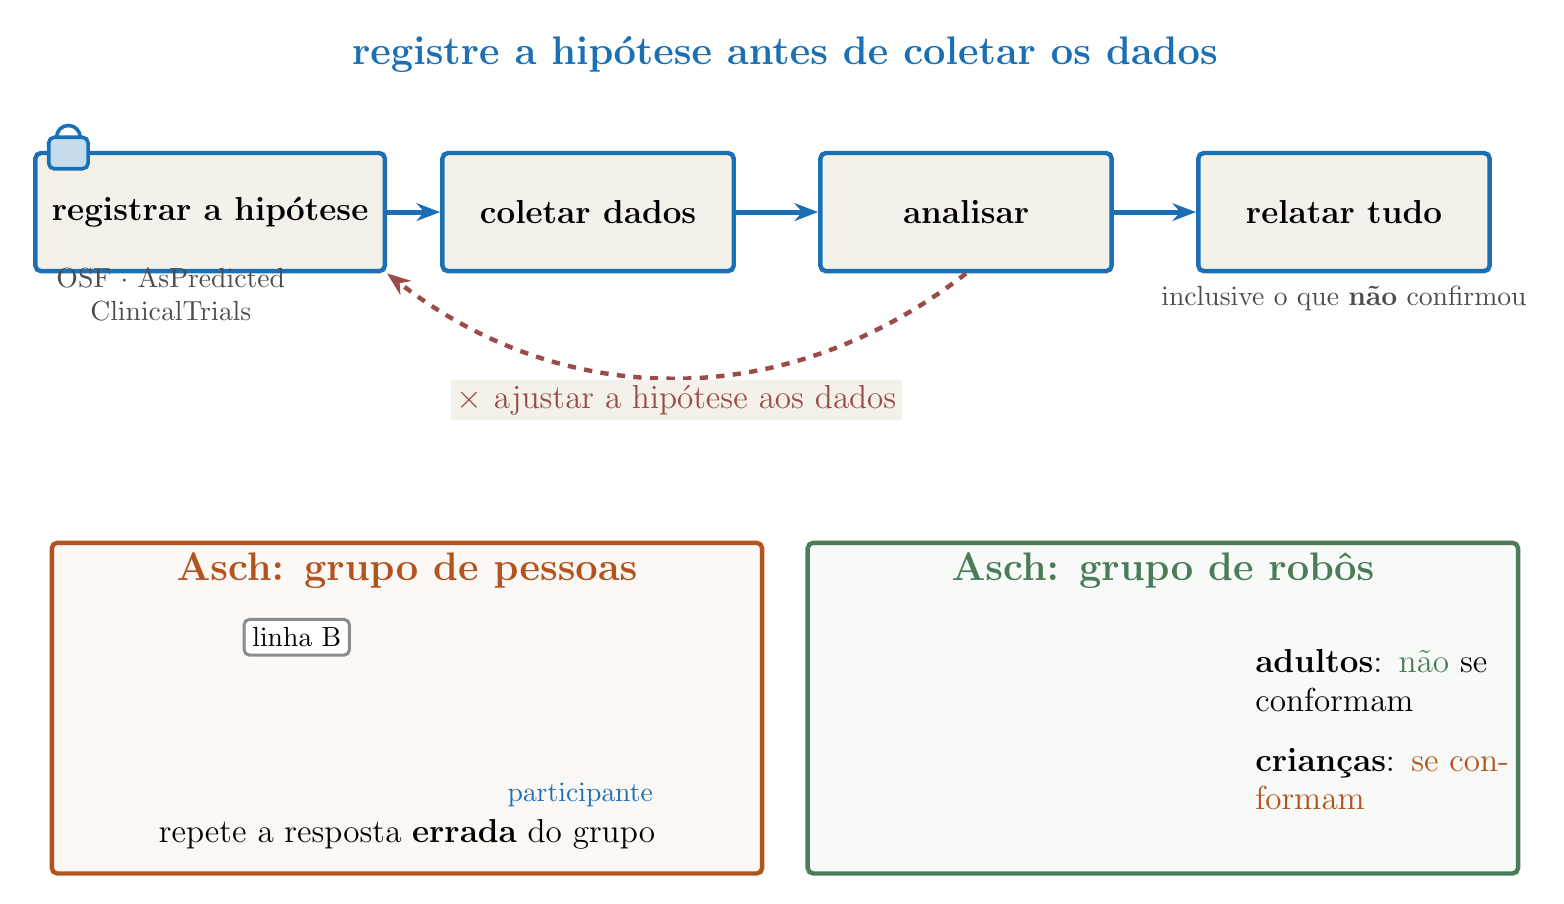
\begin{tikzpicture}[x=1cm,y=1cm]
  \tikzset{e/.style={dbox, draw=dblue, line width=1.6pt, minimum width=3.7cm, minimum height=1.5cm, font=\large\bfseries},
           bolha/.style={dbox, draw=black!45, fill=white, line width=1.1pt, font=\normalsize, inner sep=3pt}}
  % ---------- linha do tempo do registro ----------
  \node[font=\Large\bfseries, dblue] at (9.5,10.4) {registre a hipótese \textbf{antes} de coletar os dados};
  \node[e] (a) at (2.2,8.4) {registrar a hipótese};
  \node[e] (b) at (7.0,8.4) {coletar dados};
  \node[e] (c) at (11.8,8.4) {analisar};
  \node[e] (d) at (16.6,8.4) {relatar tudo};
  \draw[dtrans, line width=1.8pt, -{Stealth[length=3mm]}] (a.east) -- (b.west);
  \draw[dtrans, line width=1.8pt, -{Stealth[length=3mm]}] (b.east) -- (c.west);
  \draw[dtrans, line width=1.8pt, -{Stealth[length=3mm]}] (c.east) -- (d.west);
  % cadeado em (a)
  \draw[dblue, fill=dblue!25, line width=1.3pt, rounded corners=2pt] (0.15,8.95) rectangle (0.65,9.35);
  \draw[dblue, line width=1.3pt] (0.25,9.35) arc(180:0:0.15);
  \node[font=\normalsize, black!70, text width=3.4cm, align=center] at (1.7,7.35) {OSF $\cdot$ AsPredicted\\ ClinicalTrials};
  \node[font=\normalsize, black!70] at (16.6,7.3) {inclusive o que \textbf{não} confirmou};
  % caminho proibido
  \draw[dred, dashed, line width=1.6pt, -{Stealth[length=3mm]}] (c.south) to[bend left=38] node[midway, below, font=\large, dred, fill=dcream, inner sep=2pt] {\textbf{$\times$} ajustar a hipótese aos dados} (a.south east);
  % ---------- Asch ----------
  \node[dbox, draw=dorange, line width=1.6pt, text width=8.6cm, minimum height=4.2cm, fill=dorange!4] at (4.7,2.1) {};
  \node[font=\Large\bfseries, dorange] at (4.7,3.85) {Asch: grupo de pessoas};
  \pess{1.9}{1.9}{black!55}{black!8} \pess{3.3}{1.9}{black!55}{black!8} \pess{4.7}{1.9}{black!55}{black!8} \pess{6.9}{1.9}{dblue}{dblue!15}
  \node[bolha] at (3.3,3.0) {linha B};
  \node[font=\normalsize, dblue] at (6.9,1.0) {participante};
  \node[font=\large, text width=7.8cm, align=center] at (4.7,0.5) {repete a resposta \textbf{errada} do grupo};
  \node[dbox, draw=dgreen, line width=1.6pt, text width=8.6cm, minimum height=4.2cm, fill=dgreen!4] at (14.3,2.1) {};
  \node[font=\Large\bfseries, dgreen] at (14.3,3.85) {Asch: grupo de robôs};
  \rob{11.5}{1.9} \rob{12.9}{1.9} \rob{14.3}{1.9}
  \node[font=\large, anchor=west, text width=3.3cm, align=left] at (15.35,2.45) {\textbf{adultos}: \textcolor{dgreen}{não} se conformam};
  \node[font=\large, anchor=west, text width=3.3cm, align=left] at (15.35,1.2) {\textbf{crianças}: \textcolor{dorange}{se conformam}};
\end{tikzpicture}
\end{document}
